\documentclass[10pt,a4paper]{article}
\usepackage{algorithm}
\usepackage{algorithmicx}
\usepackage{algpseudocode}
\usepackage{amsfonts}
\usepackage{amsmath}
\usepackage{amssymb}
\usepackage{bbm}
\usepackage[a4paper, portrait, margin=1in]{geometry}
\usepackage{graphicx}
\usepackage[numbers]{natbib}
\usepackage{pdflscape}
\usepackage[utf8]{inputenc}
\author{Nathan Cunningham}
\title{MDI SMC: Progress Report}
\begin{document}
\maketitle


\section{What have I done?}
\begin{itemize}
\item Implemented the multinomial resampling step, carried out after each 'per-gene' iteration. This doesn't appear to have corrected the sensitivity of the algorithm to the ordering of the data. The \citeauthor{griffin2014sequential} \cite{griffin2014sequential} paper mentions randomly permuting the data also, ``the data were randomly permuted and the SMC algorithms was run with 5000 particles''.
\item The particle Gibbs steps is a work in progress still. The approach I'm taking is to hold one of the particles as fixed, then resample the allocation holding this reference trajectory fixed.
\item I examined the output from the original MDI on the same data as I'd tested the SMC algorithm  on. The output appears to converge quickly to complete fusion across clusters. Figures presented below.
 \item The weight updates, $\xi$, have not been changed, as I think they are being updated correctly in the code, but I might have written the math inaccurately. Algorithm updated below.
\end{itemize}




\section*{General algorithm}
\begin{algorithm}
\caption{Gibbs sampler}
 \begin{algorithmic}[1]
  \State Initialise $\Gamma$ matrix of prior allocation weights and $\Phi$ matrix of dataset concordance values
  \For{i = 1, \dots, number of iterations}
  \State Conditional on $\Gamma_{i-1}$ and $\Phi_{i-1}$ update the cluster labels, $c_{i}$, using alg. \ref{alg:pf}
  \State Conditional on $c_{i}$ update $\Gamma_i$ and $\Phi_i$
  \EndFor
\end{algorithmic}
\end{algorithm}


\begin{algorithm}
\caption{Particle filter to update cluster allocations}
\label{alg:pf}
 \begin{algorithmic}[1]
  \For{i = 1, \dots, n} \Comment{Loop over observations}
  \For{m = 1, \dots, M} \Comment{Loop over particles}
  \For{j = 1, \dots, d} \Comment{Loop over datasets}
  \State Sample $c^{(m)}_{i, j}$ \Comment{Propose a cluster for each datum}
  \State $q(c^{(m)}_{i,j} = k) \propto k^*(y_{i,j}|c_{i,j}^{(m)} = k) \times \gamma_{i, k, j}$ 

  \EndFor
    \State $\xi^{(m)} = \xi^{(m)} \times {\displaystyle\prod_{k = 1}^{d - 1}}{\displaystyle\prod_{l = k + 1}^{d}} (1+\phi_{kl} \mathbbm{1}(c_{ik} = c_{il}) {\displaystyle\prod_{j = 1}^{d}} \gamma_{i, k, j} k^*(y_{i,k}|c_{i,j}^{(m)} = k)$
  \EndFor
  \State Resample particles according to $\xi^{(m)}$
  \EndFor
  \State Select single cluster label allocation according to $\xi^{(m)}$

\end{algorithmic}
\end{algorithm}

Where
\begin{equation}
\label{eq:likelihood}
k^*(y_{i, k}|c_{i, k}^{(m)} = k) = (\mathbf{y_{i, k}} - \mathbf{\mu_k}) \mathbf{\Sigma^{-1}} (\mathbf{y_{i, k}} - \mathbf{\mu_k})^\top
\end{equation}
\begin{equation}
\label{eq:phi}
\Phi \text{ is a measure of cluster label correspondence across datasets}
\end{equation}
\begin{equation}
\label{eq:gamma}
\gamma_{i, k, j} \text{ is a prior weight for assigning observation i, in dataset k to cluster j}
\end{equation}


\begin{landscape}
\begin{figure}[htbp]
\label{fig:multinom1}
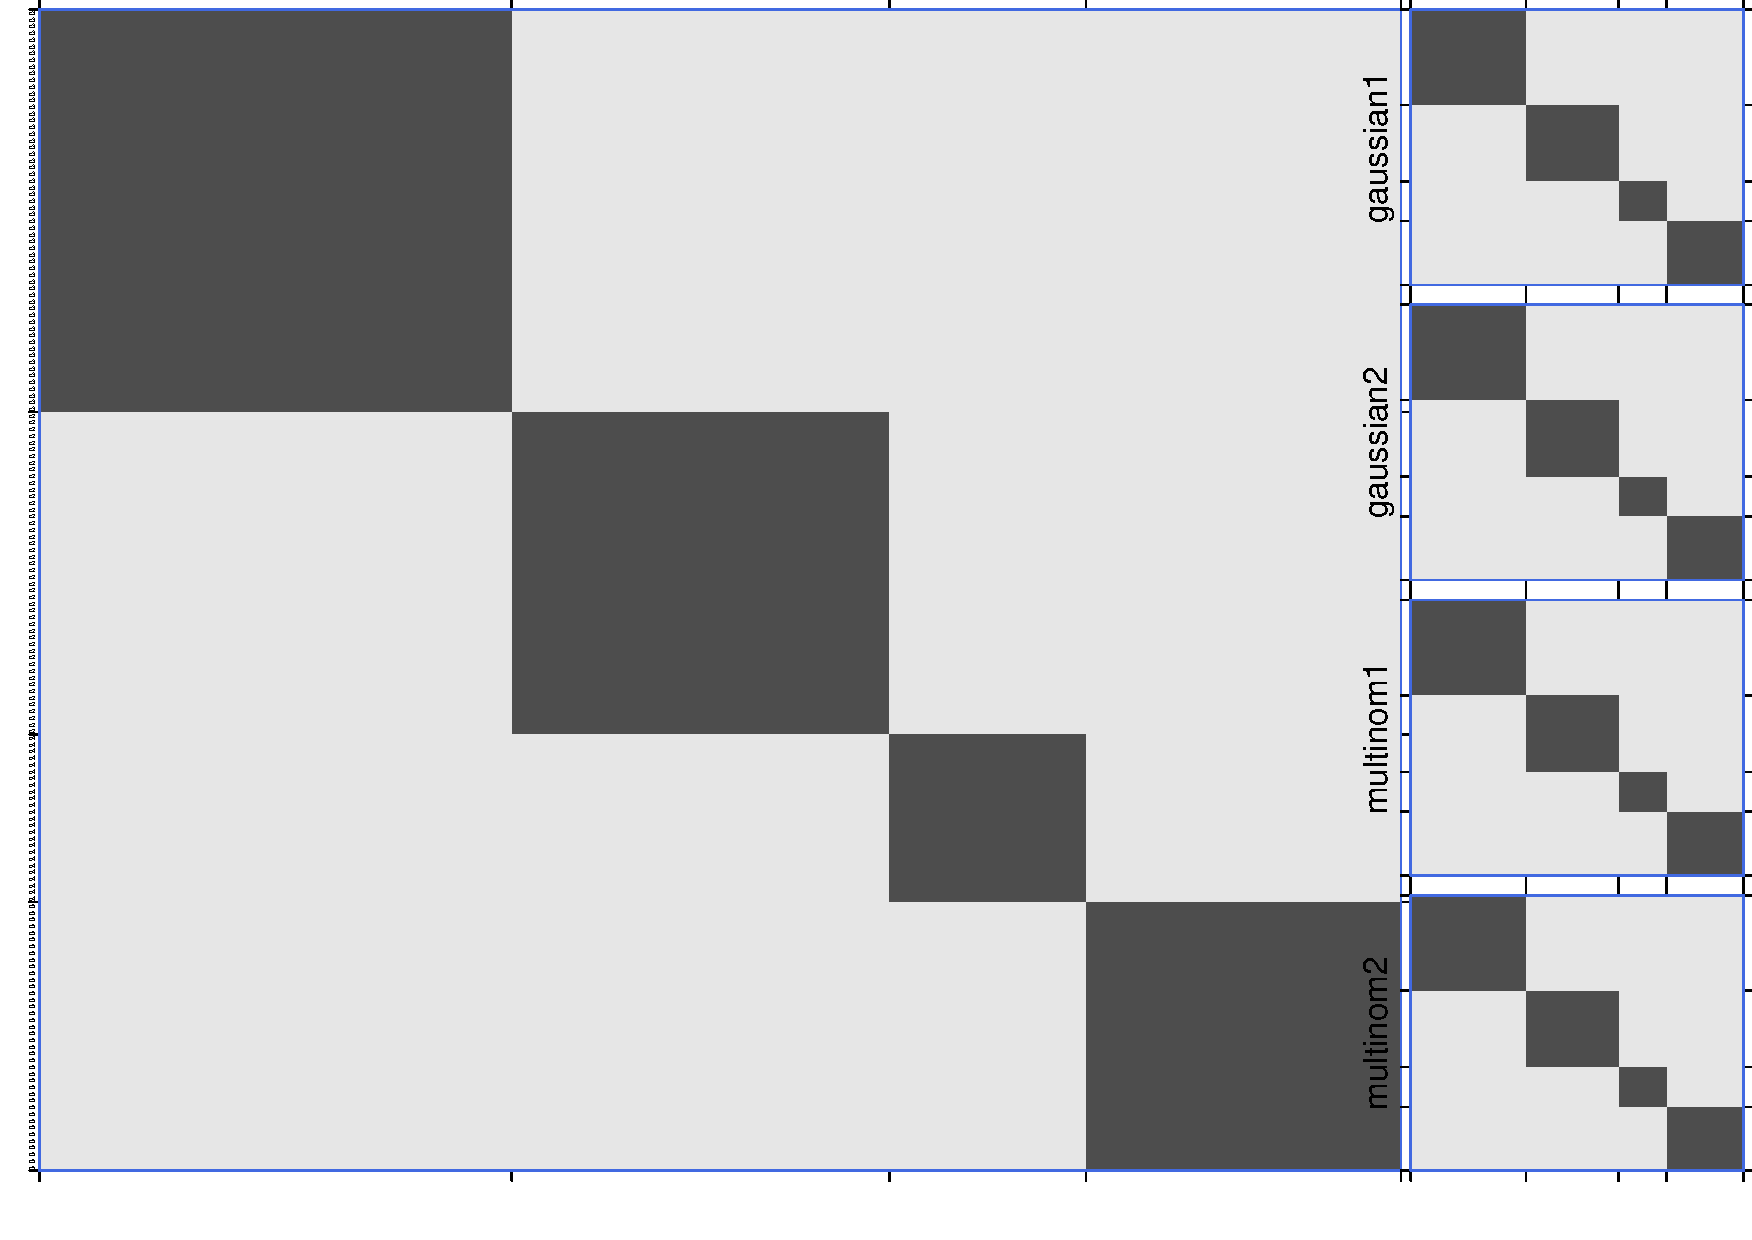
\includegraphics[width = 0.95\linewidth]{plots/mdi_orig_consensus.pdf}
\caption{Running the original MDI using four datasets: two gaussian and two multinomial, with a shared clustering order.}
\end{figure}
\begin{figure}[htbp]
\label{fig:multinom1}
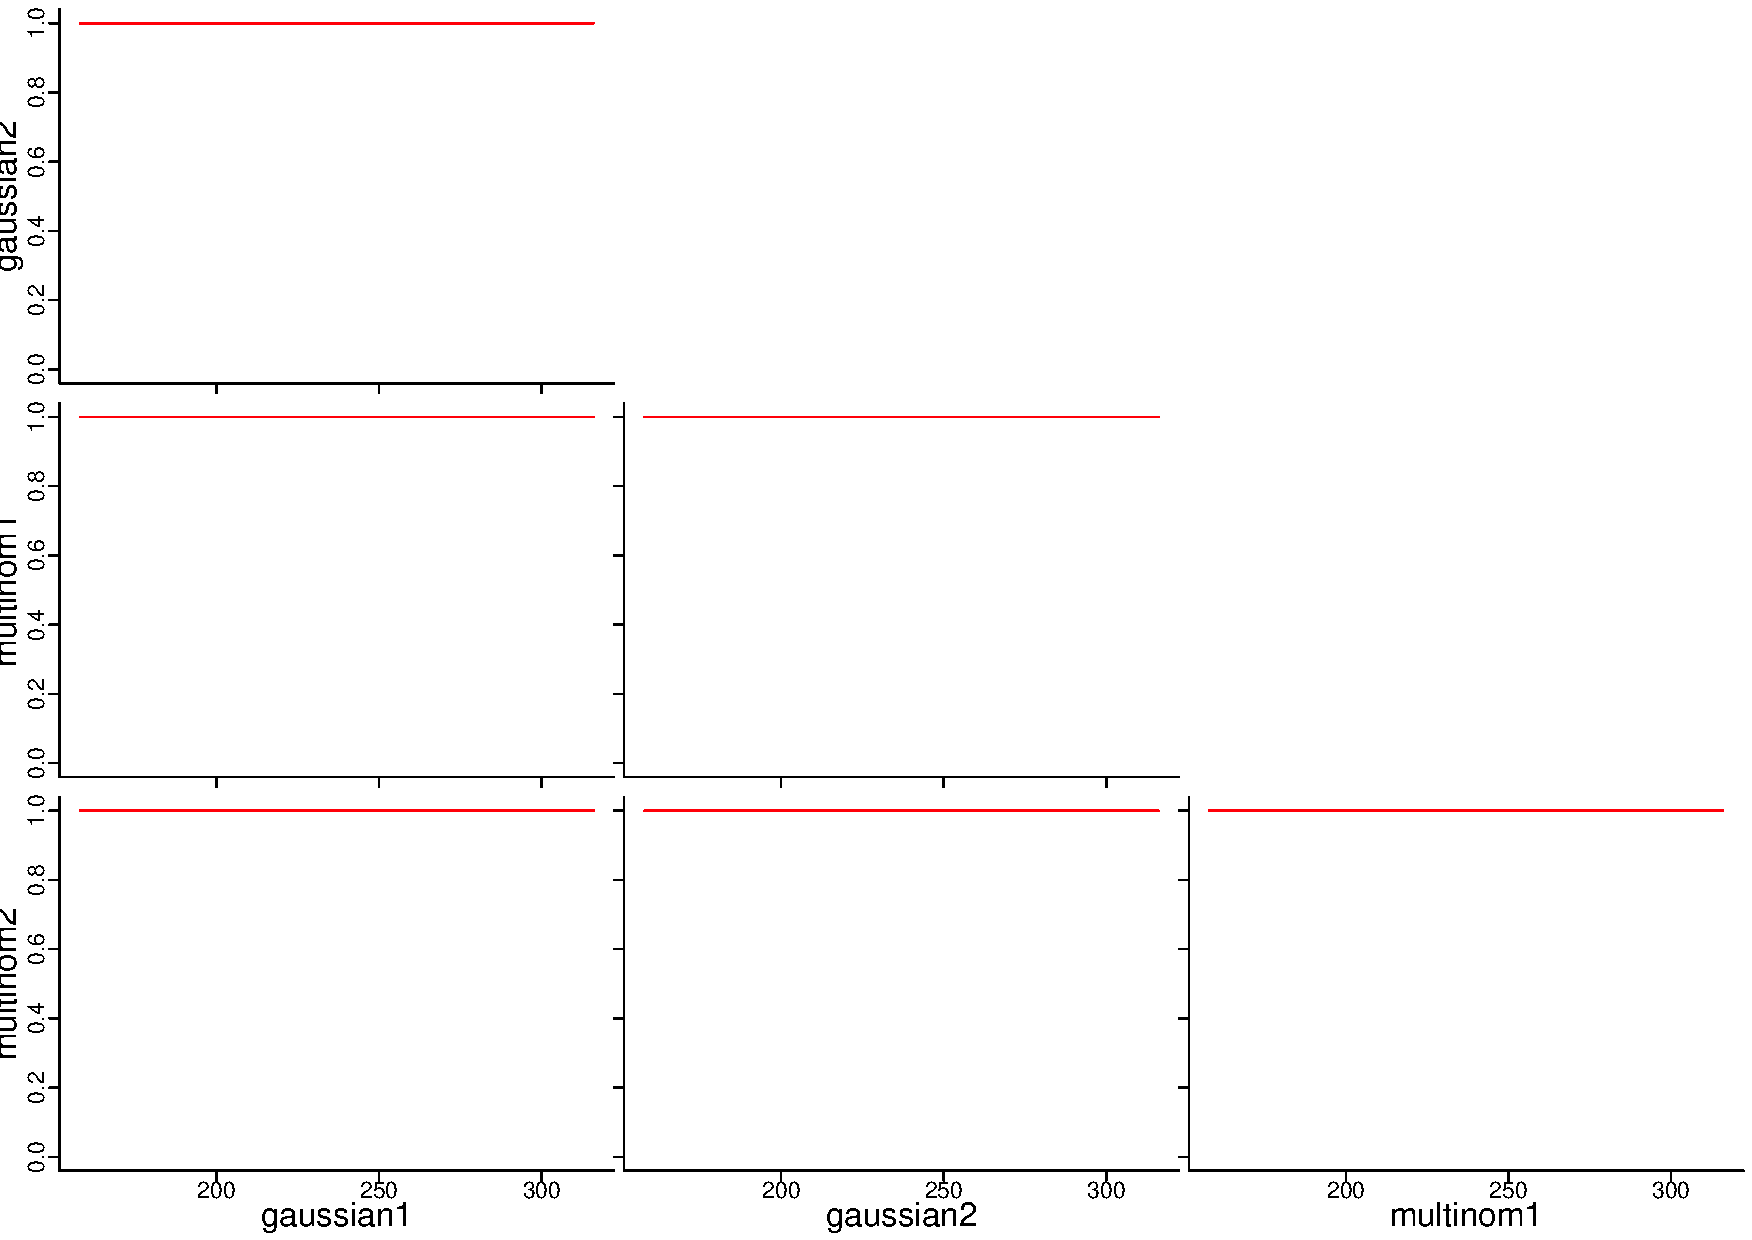
\includegraphics[width = 0.95\linewidth]{plots/mdi_orig_agreement.pdf}
\caption{Allocation agreement the original MDI using four datasets: two gaussian and two multinomial, with a shared clustering order. Genes are allocated to the same clusters across datasets.}
\end{figure}
\begin{figure}[htbp]
\label{fig:multinom1}
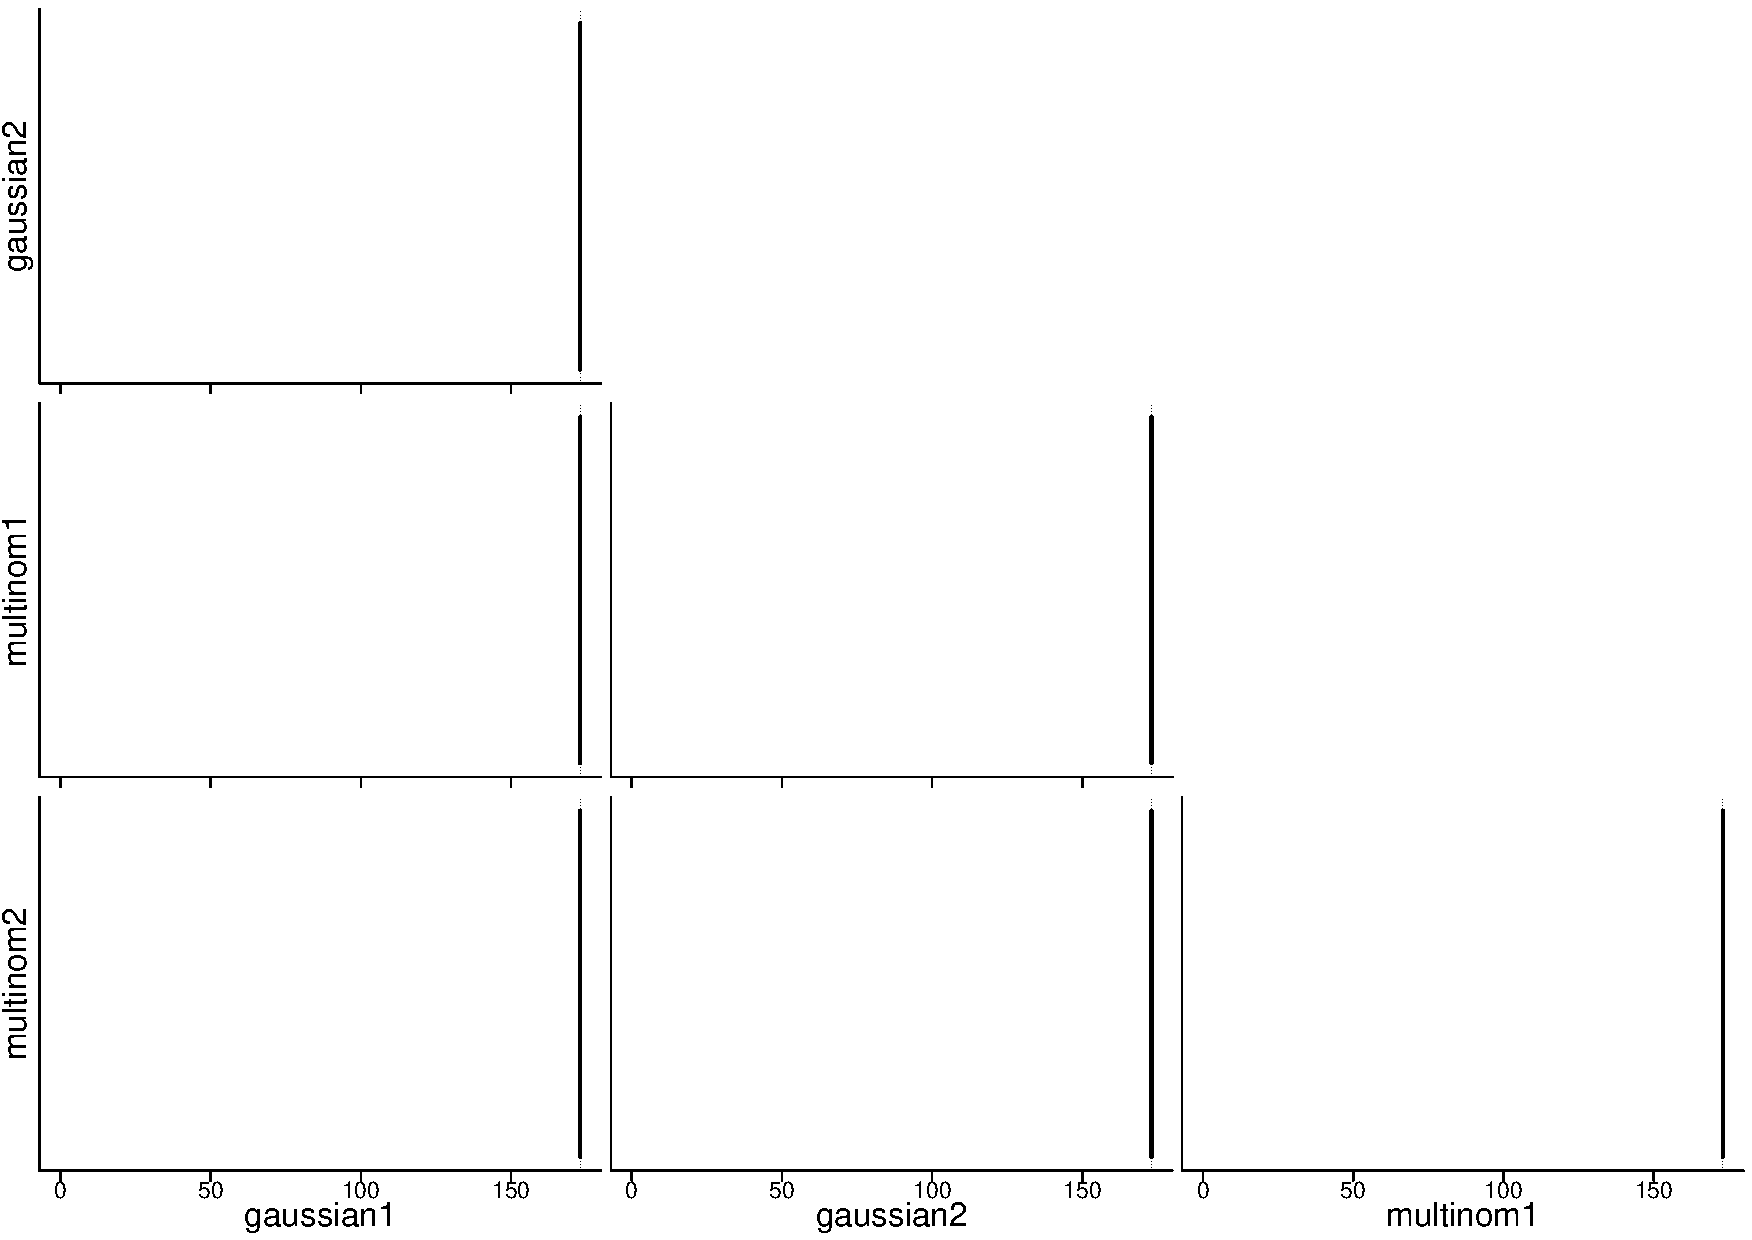
\includegraphics[width = 0.95\linewidth]{plots/mdi_orig_hist.pdf}
\caption{Allocation agreement the original MDI using four datasets: two gaussian and two multinomial, with a shared clustering order. Genes are allocated to the same clusters across datasets.}
\end{figure}
\end{landscape}

\bibliographystyle{plainnat}
\bibliography{bibliography.bib}

\end{document}